% Compile to SVG with: pdflatex -shell-escape repr_research.tex 
\documentclass[convert={outfile=reprresearch.svg}]{standalone}
\usepackage[latin1]{inputenc}
\usepackage{amsmath}
\usepackage{amsfonts}
\usepackage{amssymb}
\usepackage{tikz}
\usepackage{fontawesome}
\usetikzlibrary{calc}

\begin{document}
	\begin{normalsize}
		\begin{tikzpicture}
		
		\def\x{3.5};
		\def\y{3.5};
		\def\ys{-7};
		\definecolor{bgcolor}{RGB}{250, 250, 250}
		
		\node (pkg) at (1.5*\x, -0.5*\y) {\faFileCodeO};
		
		\node (raw) at (0, -\y) {\faFileArchiveO};
		
		\node (tidy-d) at (1.5*\x, -\y) {\faFileTextO};
		\node (plot-pdf) at (3*\x, -0.5*\y) {\faFilePdfO};
		\node (table-tex) at (3*\x, -1.5*\y) {\faFileTextO};
		
		\coordinate (tidy-f) at ($(raw)!0.5!(tidy-d)$);
		\coordinate (create-data) at ($(tidy-d)!0.5!(plot-pdf)$);
		\coordinate (create-table) at ($(tidy-d)!0.5!(table-tex)$);
		
		\draw [->] (raw) -- (tidy-d) node [pos=0.5,above,sloped] {\faFileCodeO \ tidy\_data()};
		\draw [->] (tidy-d) -- (plot-pdf) node [pos=0.5,above,sloped] {\faFileCodeO \ create\_plot1()};
		\draw [->] (tidy-d) -- (table-tex) node [pos=0.5,above,sloped] {\faFileCodeO \ create\_table1()};
		
		
		\draw [->, dashed] (pkg) -- ([yshift=15]tidy-f);
		\draw [->, dashed] (pkg) -- ([yshift=15]create-data);
		\draw [->, dashed] (pkg) -- ([yshift=15]create-table);
		
		% create_functions
		
		% tex-files
		\node (main-tex) at (4*\x, -1*\y) {\faFileTextO};
		
		\node (main-pdf) at (5*\x, -\y) {\faFilePdfO};
		
		draw [->] (raw) -- (tidy-d);
		\draw [->] (plot-pdf) -- (main-tex);
		\draw [->] (table-tex) -- (main-tex);
		\draw [->] (main-tex) -- (main-pdf);
		
		\node at (raw) [anchor=north,yshift=\ys] {raw\_data.csv};
		\node at (tidy-d) [anchor=north,yshift=\ys] {tidy\_data.csv};
		\node at (plot-pdf) [anchor=north,yshift=\ys] {plot1.pdf};
		\node at (table-tex) [anchor=north,yshift=\ys] {table1.tex};
		\node at (main-tex) [anchor=north,yshift=\ys] {main.tex};
		\node at (main-pdf) [anchor=north,yshift=\ys] {main.pdf};
		\node at (pkg) [anchor=north,yshift=\ys] {myPkg};
		
		
		
		
		%\draw (0,0) node {\faFileTextO};
		%\draw (0,-\dx) node {raw\_data.csv};
		%\draw[->] (\dx,0) -- (\x-\dx,0); % raw to data_munging
		%
		%\draw (\x,0) node {\faFileCodeO};
		%\draw (\x,-\dx) node {tidy\_data()};
		%\draw[->] (\x,-2*\dy) -- (\x,-\y+\dx); % data_munging to tidy
		%
		%\draw (\x,-\y) node {\faFileTextO};
		%\draw (\x,-\y-\dy) node {tidy\_data.csv};
		%\draw[->] (\x+\dx,-\y-1.75*\dy) -- (2*\x-\dx,-2*\y+\dy); % tidy data to table1
		%\draw[->] (\x+\dx,-\y) -- (2*\x-\dx,-\y); %tidy_data to plot1
		%
		%\draw (2.5*\x,0) node {\faFileCodeO};
		%\draw (2.5*\x,-\dy) node {myPackage};
		%\draw[<-, dashed] (\x+\dx,0) -- (2.5*\x-\dx,0); % functions to data_munging
		%\draw[<-, dashed] (2*\x+\dx,-\y+\dy) -- (2.5*\x,-1.75*\dy); % functions to plot1
		%\draw[<-, dashed] (2*\x+\dx,-2*\y+\dy) -- (2.5*\x,-1.75*\dy); % functions to table1
		%
		%\draw (2*\x,-\y) node {\faFileCodeO};
		%\draw (2*\x,-\y-\dy) node {create\_plot1()};
		%\draw[->] (2*\x+\dx,-\y) -- (3*\x-\dx,-\y); % plot1 to plot1
		%
		%\draw (3*\x,-\y) node {\faFileCodeO};
		%\draw (3*\x,-\y-\dy) node {plot1.pdf};
		%
		%\draw (2*\x,-2*\y) node {\faFileCodeO};
		%\draw (2*\x,-2*\y-\dy) node {create\_table1()};
		%\draw[->] (2*\x+\dx,-2*\y) -- (3*\x-\dx,-2*\y); % table1 to table1
		%\draw (3*\x,-2*\y) node {\faFileCodeO};
		%\draw (3*\x,-2*\y-\dy) node {table1.tex};
		%
		%\draw (4*\x,-1.5*\y) node {\faFileCodeO};
		%\draw (4*\x,-1.5*\y-\dy) node {main.tex};
		%
		%
		%\draw (5*\x,-1.5*\y) node {\faFilePdfO};
		%\draw (5*\x,-1.5*\y-\dy) node {main.pdf};
		%\draw[->] (4*\x + \dx,-1.5*\y) -- (5*\x-\dx,-1.5*\y);% main to main
		%
		%\draw[->] (3*\x+\dx,-\y) -- (4*\x-\dx,-1.5*\y+\dy); % plot1 to main
		%\draw[->] (3*\x+\dx,-2*\y) -- (4*\x-\dx,-1.5*\y-2*\dy); % table1 to main
		
		\end{tikzpicture}
	\end{normalsize}
\end{document}